\chapter{Introduction}
\label{chapter:introduction}
Software engineering is becoming an increasingly challenging task nowadays. Developing software with complex architectures and nontrivial implementations is a prevalent task for the modern software engineer, having implications on how software is developed. At the same time, software that can be proven to be error-free has become increasingly important. The reason for this is apparent. Sophisticated systems automate more and more crucial tasks. Failure of these systems might have enormous consequences, especially for safety-critical and healthcare systems. Therefore, multiple strategies have been developed over the years to ensure that crucial parts of these systems are error-free.

An increasingly popular method for dealing with the development of complex systems is by using domain-specific models. Model-Driven Engineering (MDE) is a field within software engineering that focuses on using and creating domain models that describe complex software systems on a domain level. These models can then be used for different tasks, depending on the type of model. These tasks include code generation, but also different forms of verification of the software. By using these models, it becomes easier to reason about the developed software, while also allowing for systematic code generation and verification.

Although domain-specific models provide a strategy to deal with the development of complex systems, they do not automatically ensure that the software is error-free. Software verification is an essential strategy in ensuring that software systems are error-free. Modern methods of software verification use automated tools that can use software models to verify the correctness of a system. These tools use some model of the system to verify a set of requirements provided by the software engineer. By using structural checks on the model, the tool can tell if these requirements are met.

A possible problem that might arise when using domain-specific models for software development is the interoperability of different models. Within the area of MDE, a lot of different frameworks and tools exist. Each of these frameworks and tools focuses on a specific set of functionality. As a result, models created in one framework well suited for code generation, might not be useful in the context of software verification. In an ideal world, the format of the produced models would be standardised across all frameworks for smooth interoperability. In reality, different frameworks use different formats which are optimised for their specific set of functions. These different formats make it difficult to share models across different frameworks and applications.

Model transformation is a concept in the field of MDE that focuses on solving this problem. Model transformation is an automated way of modifying and creating models by transforming existing models. By using model transformations, it is possible to transform a model that is tailored towards code generation into a model that is suited for software verification, without the need to create a new model for this purpose.

Model transformations have already led to various tools and services that can export and import models in different tools and frameworks. These tools and services allow a software engineer to transform a model suited for code generation into a model suited for verification, and therefore use one model and its transformations to achieve both tasks. Sadly, these model transformations rarely have a formal foundation. Having a formal foundation for the model transformations is useful in the context of software verification since it allows for proving the correctness of the transformation itself. When a transformed model is used to verify a software system, the results of the verification can only be considered correct if the transformation is correct. Without proof of correctness of the transformation, it might be that the verification results are incorrect because the original model might have a different meaning than the transformed model.

This thesis will contribute to fields of MDE and Software Verification by specifying a formal foundation for model transformations between EMF/Ecore (\cref{sec:background:eclipse_modeling_framework}), a framework for software modelling in which various models can be created, and GROOVE (\cref{sec:background:groove}), a tool for software verification based on graph grammars. Furthermore, a framework is presented in which these model transformations can be proven correct, allowing the user to build correct model transformations iteratively.

\section{Formalisation of model transformations}
\label{sec:introduction:formalisation_of_model_transformations}
As explained earlier, model transformations are an automated way of modifying and creating models by transforming existing models. Model transformations can be used in a variety of scenarios, from simple modifications within the same domain and language (an endogenous transformation) to conversions between different domains and languages (an exogenous transformation). Furthermore, model transformations can be unidirectional, meaning that a model can only be transformed one way, or bidirectional, meaning that the model can be transformed in both directions. Unidirectional transformations are particularly useful in situations where the output model is meant to be used as a final result, such as code generation. Bidirectional transformations are necessary for situations where the models must be kept consistent. In that case, a change to one model might necessitate a change to the other model, which then can be automated using model transformations.

Since this thesis focuses on model transformations between EMF/Ecore and GROOVE, this thesis focuses on bidirectional exogenous transformations. The transformations between EMF/Ecore and GROOVE are exogenous by definition, since the languages of EMF/Ecore and GROOVE are different, as will be shown later. The bidirectionality of the transformations is beneficial to ensure consistency, which is a useful property to have in software verification.

In order to prove any property on these model transformations, the transformations need to be formalised. The formalisation of a model transformation consists of mathematical definitions and functions that describe the behaviour of the transformation, allowing to mathematically translate an input model to an output model as described by the model transformation. These definitions and functions directly depend on the formalisations of the input and output models themselves, as these are needed to describe the input and output models of the transformations. Because of this dependency, the formalisations of EMF/Ecore and GROOVE must be established as well.

The main disadvantage of the formalisation of model transformations is the direct relationship between the transformation and its input and output language. As a consequence, the formalisation of a model transformation directly depends on the formalisations of its input and output languages. Therefore, it is not possible to give an abstract formalisation for model transformations between different languages. Creating such a formalisation would mean making the formalisations of the input and output languages more abstract. Making these more abstract might result in loss of information, which is undesirable, or an increase in complexity. Within this thesis, this disadvantage was dealt with by only focusing on the model transformations between EMF/Ecore and GROOVE.
\section{Correctness of model transformations}
\label{sec:introduction:correctness_of_model_transformations}

As explained in \cref{sec:introduction:formalisation_of_model_transformations}, this thesis will define a formalisation for model transformations from EMF/Ecore to GROOVE and vice versa. However, a formalisation of the transformation itself does not prove anything about its properties and correctness. In order for the formalisation of the model transformation to be useful in the context of software verification, it is essential to prove its correctness. Therefore, it is crucial to establish what it means for a model transformation to be correct.

As explained earlier, the model transformations between EMF/Ecore and GROOVE are exogenous and bidirectional. This bidirectionality means that for every transformation from EMF/Ecore to GROOVE, there exists a transformation back, from GROOVE to EMF/Ecore. Since GROOVE and EMF/Ecore are very different, there are elements in EMF/Ecore that cannot be expressed in GROOVE and vice versa. Because of the difference, it might not be possible to use one mapping in both directions. Therefore, it might be the case that for a transformation from EMF/Ecore to GROOVE, a different transformation function is used to convert the model back from GROOVE to EMF/Ecore. In this case, two unidirectional transformations are used to achieve bidirectionality.

Throughout this thesis, the correctness of a model transformation is defined as the syntactical correctness. The semantics are not further discussed as the semantics might differ from model to model, depending on what the creator intended to model. The following properties must hold for the formalisation for it to be correct. Please note that since GROOVE is based on graph grammars, one does not speak of a GROOVE model, but rather a GROOVE graph:
\begin{itemize}
    \item For each valid EMF/Ecore model that is transformed to GROOVE, the resulting GROOVE graph must be syntactically valid.
    \item For each valid GROOVE graph that is transformed to EMF/Ecore, the resulting EMF/Ecore model must be syntactically valid.
    \item For each valid EMF/Ecore model that is transformed to GROOVE, there exists a known transformation from the resulting GROOVE graph back to the original EMF/Ecore model.
    \item For each valid GROOVE graph that is transformed to EMF/Ecore, there exists a known transformation from the resulting EMF/Ecore model back to the original GROOVE graph.
\end{itemize}

These properties assume that it is clear what it means for EMF/Ecore models and GROOVE graphs to be syntactically valid. Therefore, the formalisations of EMF/Ecore and GROOVE will specify the syntactical correctness of their models and graphs.

The properties discussed above are useful in the context of software verification since they show that the transformed models and graphs are indeed a valid transformation of their original counterparts. Therefore, this thesis will not only define the formalisation for the model transformations but also show that the properties discussed above hold for these transformations.
\section{Approach and composability}
\label{sec:introduction:approach}

As explained in the previous sections, this thesis will provide a formalisation for the model transformations between Ecore and GROOVE and also prove the correctness of the transformations. Although this a noble goal, it comes with many complexities.

First of all, Ecore and GROOVE both have a very different nature. Ecore is mostly based on a subset of UML, as discussed in \cref{sec:background:eclipse_modeling_framework}. On the other hand, GROOVE is based around graph grammars and therefore mathematical graph theory. As a consequence, the set of features is very different. Ecore has elements that are not directly expressable in GROOVE and vice versa. When providing the formalisation for the transformations, the different features within both languages should be taken into account.

Furthermore, Ecore and GROOVE have a lot of different elements within their models and grammars. When transforming these models and grammars, all these elements need to be transformed. Transforming all these elements at once is a very complex problem, as these different elements can be used in infinitely many combinations, each requiring a different transformation. Not only must the formalisation be able to express all these different combinations, but each of these combinations must also be proven correct.

In order to overcome the problems that are raised by these complexities, the divide and conquer-principle will be applied. This thesis will provide a framework in which model transformations and their proofs can be composed out of smaller transformations and their proofs. This composability allows for proving only small parts of the problem, which then can be composed to express the countless combinations of model transformations.
\section{Research question}
\label{sec:introduction:research_question}
This thesis will focus on defining a formalisation for model transformations from Ecore to GROOVE and vice versa, and also proving the correctness of these transformations. It will try to achieve this goal by providing a way to compose more substantial model transformations out of smaller ones. In short, the thesis will answer the following research question:

``What is a suitable formalisation for composable model transformations between Ecore and GROOVE that gives rise to correct model transformations between Ecore and GROOVE?''

It is immediately clear that this research question consists of multiple facets. In order to make answering the research question easier, the research question will be split into smaller questions based on the different facets of the main question. The following subquestions will be answered:
\begin{enumerate}
    \item ``What is a suitable formalisation of Ecore models and what Ecore models are valid within this formalisation?'' 
    
    In order to transform between Ecore and GROOVE, a formalisation of Ecore is needed. As explained earlier, this formalisation needs to give rise to a definition of valid Ecore models, which are needed to prove the correctness of the transformations later.
    
    \item ``What is a suitable formalisation of GROOVE grammars and what GROOVE grammars are valid within this formalisation?'' 
    
    Just like the previous question, a formalisation that captures GROOVE grammars is needed. Like the previous question, this formalisation should also give rise to a definition of valid GROOVE grammars for use in proving the correctness of the transformations.
    
    \item ``What is a suitable formalisation for the model transformations between Ecore and GROOVE?'' 
    
    A suitable formalisation for the model transformations between Ecore and GROOVE is needed to describe the model transformations between Ecore and GROOVE formally. Such a formalisation must be able to express the infinite combinations of possible model transformations. This formalisation forms the basis of the correctness of model transformations and their composability. Therefore, this question is the foundation of the main result of this thesis.
    
    \item ``What model transformations are correct within the formalisation?'' 
    
    This question will answer the question which model transformations within the formalisation are correct model transformations between Ecore and GROOVE. These transformations are of interest, as only these transformations can be used with confidence within formal applications.
    
    \item ``How can correct model transformations between Ecore and GROOVE be composed?''
    
    A fundamental part of this thesis is to compose small model transformations into larger ones. This composability allows for only proving the correctness of small model transformations and then combining them without loss of correctness. This question answers how to compose correct model transformations into a new model transformation while preserving correctness.
\end{enumerate}

When these subquestions are answered, it is possible to formulate an answer to the main research question. A suitable formalisation for model transformations between Ecore and GROOVE will follow from subquestions 1, 2 and 3. Subquestions 1 and 2 provide the formalisations of Ecore and GROOVE themselves, which will be used to formalise their model transformations. Subquestion 3 defines the formalisation of the model transformations. The correctness of model transformations within this formalisation will follow from subquestions 1, 2 and 4. Subquestions 1 and 2 will provide the definitions needed to prove correctness, while subquestion 4 will give a proof for the correct model transformations. Finally, the composability of these model transformations follows from subquestion 5, which answers how to combine correct model transformations while preserving correctness.
\section{Validation}
\label{sec:introduction:validation}
This section describes how the research questions of this thesis will be validated. The main research question of this thesis will be validated by validating the subquestions. For each subquestion, the validation process is different:
\begin{itemize}
    \item ``What is a suitable formalisation of Ecore models and what Ecore models are valid within this formalisation?'' and ``What is a suitable formalisation of GROOVE grammars and what GROOVE grammars are valid within this formalisation?''
    
    The answer to these questions will be validated through existing theory about these modelling languages. Existing theories describe the different elements in these languages and the constraints between them. These give rise to domains for both languages, which can be used to formalise the language. The correctness of the grammars and models in these languages follow from literature in the same way, as the literature defines which grammars and models are valid within these languages.
    
    \item ``What is a suitable formalisation for the model transformations between Ecore and GROOVE?'' 
    
    A suitable formalisation must be able to express a reasonable set of model transformations. If the formalisation is not able to express such a set, the formalisation is useless. Therefore, the thesis will show examples of model transformations within this formalisation and give an intuition of which transformations are possible. The existence of these examples validates the suitability of the formalisation.
    
    \item ``What model transformations are correct within the formalisation?'' 
    
    The correctness of the model transformations follows from a correctness proof. This proof is validated using a theorem prover, which ensures that the proof is sound and complete. Therefore, the theorem prover validates the proof, while the proof validates the answer to the question. Furthermore, examples of correct model transformations will be provided, which validates that correct model transformations exist within the formalisation.
    
    \item ``How can correct model transformations between Ecore and GROOVE be composed?''
    
    This subquestions answers how correct model transformations can be composed such that the result is also correct. Validating this question consists of two parts. In the first part, a correctness proof is given, which shows that the composed model transformations are indeed a correct model transformation itself. This correctness proof is validated using a theorem prover. In the second part, an application of the composability of model transformations is shown, which validates that composing model transformations is possible in practice.
\end{itemize}

Since the answer to the main research question follows directly from the answers to the subquestions, the answer to the main question is validated using the validation of the subquestions.
\section{Related work}
\label{sec:introduction:related_work}
In this section, the work related to this thesis will be discussed. The related work is divided into multiple sections that each describe a different facet related to this thesis.


\subsection{Formalisations of modelling languages}
\label{subsec:introduction:related_work:formalisations_of_modelling_languages}
This section discusses some related work in the field of formalisations of modelling languages. The work presented here is relevant to this thesis as the formalisations of Ecore and GROOVE have an essential role throughout this thesis.

In \cite{kleppe_uml-graph-semantics}, Kleppe and Rensink present a straightforward formalisation of UML models using graph theory and graph constraints. Since Ecore is many facets similar to UML, this formalisation provides a reasonable basis for formalising Ecore as well. Such formalisation has an advantage that it is already built upon graph theory, which allows for an easy formalisation of the transformation to other graph languages. Although the work presented does include formalisations for most relevant elements of UML models, it does not have enough expressive power to formalise concepts unique to Ecore. Within this thesis, a formalisation of Ecore is used that is much closer to the Ecore implementation, with enough expressive power to formalise all the relevant concepts.

Within UML, it is possible to describe a model and its constraints using the Object Constraint Language (OCL) \cite{ocl_spec_2014}. Most queries and invariants written in OCL can also be applied to Ecore models. Moreover, EMF has its declarative language EMF-\textsc{IncQuery} \cite{emf_incquery-guindon_2016}, which can handle complex constraints that cannot be expressed using OCL. 

In \cite{semerath-validation_dsl}, Semeráth et al. present a way to formalise EMF/Ecore by expressing a subset of OCL and EMF-\textsc{IncQuery} in first-order logic. Within this work, each Ecore model is expressed as multiple sets of named elements. These elements are constrained by OCL and EMF-\textsc{IncQuery} invariants, expressed in first-order logic. The goal is to use automated reasoners to analyse the models automatically. Because OCL and EMF-\textsc{IncQuery} are more expressive languages than first-order logic, approximations are used where necessary.

The work presented by Semeráth et al. has a particular relation to this thesis since they try to formalise Ecore to be able to perform formal verification on the Ecore models. In a way, this goal is similar to the goal of this thesis, but the approach is different. Instead of formalising Ecore with the goal of verification, formalising Ecore is in this thesis merely a tool for providing a formalisation of model transformations to GROOVE. Verification is achieved through GROOVE, which is developed solely for this purpose.


\subsection{Formalisations of model transformations}
\label{subsec:introduction:related_work:formalisations_of_model_transformations}
This section discusses related work in the field of formalisations of model transformations. Existing work in this field that is relevant is mostly related to the concept of a Triple Graph Grammar (TGG). Whereas a Graph Grammar can be used to describe the evolution of a single graph model, TGGs allow for describing the relation between two graph models and also allow for transforming one kind of model to the other \cite{KW07_ag}. The formal description of model transformations using TGGs is especially relevant to this thesis, as this thesis will also formalise a specific set of model transformations.

In \cite{hermann_ehrig_golas_orejas_2014}, Hermann, Ehrig, Golas, and Orejas approach the problem of formal analysis of model transformations using triple graph grammars. They explain how triple graph grammars can be used to describe model transformations and which problems arise when performing this task. Properties related to the syntactical correctness, functional behaviour and information preservation are discussed.

The work of Hermann, Ehrig, Golas, and Orejas discusses model transformations on a more abstract level than this thesis, by providing mathematical properties and mathematical structures to approach the problem. These structures and properties are not applied to specific modelling languages. In this thesis uses a more practical approach where Ecore models are transformed to GROOVE graph grammars and vice versa. This approach allows for a mathematical specification that is tailored for these modelling languages and can, therefore, discuss specific properties of these languages in detail.

An application of TGGs on the model transformation of Ecore models is shown by \cite{biermann_ermel_taentzer_2011}. In this work, Biermann, Ermel, and Taentzer use TGGs to formalise the behaviour of model transformations between EMF models. This formalisation is done by formalising EMF models as graph grammars first and then using these graph grammars as part of the TGGs for formalising model transformations within EMF. Ermel, Hermann, Gall, and Binanzer later use this work in \cite{ermel-visual_analysis} to create an Eclipse plugin that can describe model transformations between Ecore diagrams visually, including the possibility to edit them.

The work presented by Biermann, Ermel, and Taentzer uses a formalisation of EMF to describe model transformations formally. This formalisation is similar to the work presented by this thesis but focuses on endogenous transformations (transformations between EMF models) instead of exogenous transformations (transformations from Ecore to GROOVE, in case of this thesis).

In \cite{bruintjes_bridging-groove}, Bruintjes has worked on mapping multiple languages to GROOVE and back using an intermediate conceptual model. This intermediate conceptual model can express Ecore diagrams as well, and therefore Bruintjes provides an implementation of model transformations between Ecore and GROOVE. Because the approach of this work focuses on the implementation, the model transformations are not formalised in this work. It is still worth mentioning because it is the only work that has a focus on transformations between Ecore and GROOVE specifically. Moreover, the conceptual model used within this work does not use graph grammars as a basis, which provides more freedom in expressing specific properties of Ecore.

The work presented by Bruintjes uses a similar approach for formalising Ecore models itself. This thesis will a formalisation inspired by this work, which is like the work of Bruintjes not based on graph grammars. It differs from the work of Bruintjes by focusing on the formal foundation rather than the implementation. Moreover, this thesis only focuses on the model transformations between Ecore and GROOVE, rather than multiple languages and GROOVE.
\section{Contribution}
\label{sec:introduction:contribution}

This section discusses the intended contribution of this thesis to the active field of research. This thesis will propose a transformation framework for bidirectional transformations between EMF/Ecore and GROOVE. This transformation framework makes it possible to compose transformations while maintaining a formal proof of its syntactical correctness. As discussed in \cref{sec:introduction:related_work}, most active research uses Triple Graph Grammars to deal with the problem of the formalisation of model transformations. This thesis will take a different approach by not modelling EMF/Ecore as a graph language, but rather using a more specific formalisation. Therefore, the formalisation of the transformations will not be based on Triple Graph Grammars, but it will borrow some similar concepts.

Within this work, there will be a focus on the transformations between EMF/Ecore and GROOVE. No earlier work exists that focuses on the formalisation of the transformations between these languages specifically. Because of the focus on these two languages, a practical approach can be used that results in a framework that can be used to create transformations between these two languages directly. Within existing work, either a more abstract method is used, or the formalised transformations are endogenous (e.g., in the work of Biermann, Ermel, and Taentzer \cite{biermann_ermel_taentzer_2011}).

The result of this work can be a valuable foundation for verifying Ecore software models within GROOVE. Furthermore, it could be a valuable contribution to the field of formalised model transformations in general, since it uses an approach different than using TGGs for achieving a formalisation of exogenous transformations.
\section{Outline}
\label{sec:introduction:outline}
Within this thesis, a framework for formalising model transformations will be provided, including examples and applications. In \cref{chapter:background}, more information on EMF/Ecore and GROOVE is provided. Furthermore, the theorem prover that is part of validating the proofs is introduced. In \cref{chapter:formalisations}, the formalisations of Ecore and GROOVE are introduced.
In \cref{chapter:transformation_framework}, a framework is introduced for formally expressing composable model transformations. As a part of this chapter, the formalisation of model transformations between Ecore and GROOVE is introduced. The chapter also introduces the definitions needed to compose these model transformations. \cref{chapter:library_of_transformations} introduces a non-exhaustive library of model transformations within this framework with corresponding proofs, which provides examples of the model transformations, which can be expressed within this framework. Furthermore, \cref{chapter:application} shows the composability of these model transformations by providing an example of composing smaller model transformations in a practical example. Finally, \cref{chapter:conclusion} concludes the thesis by answering the research questions and discussing possible future work.

\subsection{Mathematical notation}
\label{subsec:introduction:outline:mathematical_notation}
Throughout this thesis, a lot of mathematical definitions and proofs are introduced. In order to accommodate for these definitions and proofs, prior knowledge of commonly used mathematical notations is assumed. For completeness, the meaning of the different braces and parentheses is as follows:
\begin{itemize}
    \item Braces, ``$\{\}$'', are used to denote mathematical sets;
    \item Angle brackets, ``$\langle \rangle$'', are used to denote mathematical sequences and named tuples;
    \item Parentheses, ``$()$'', are used to denote unnamed tuples or grouping within expressions.
\end{itemize}
Besides commonly used notations, new notations are introduced as part of some definitions throughout this thesis.

\subsection{References to validated proofs}
\label{subsec:introduction:outline:references_to_validated_proofs}
As explained \cref{sec:introduction:validation}, the formal proofs within this thesis will be validated using a theorem prover. In order to easily find the validated proofs corresponding to definitions and theorems, all relevant definitions and theorems will include a reference to the validated proof. Such a reference can be recognised by the 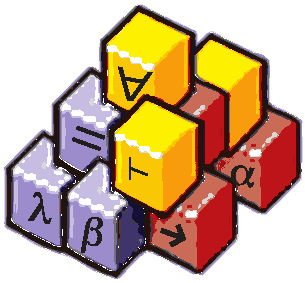
\includegraphics[height=0.75\baselineskip,keepaspectratio]{images/isabelle_logo.pdf} symbol and includes the corresponding name of the definition or theorem. For example, a reference to the theorem $mult\!\_zero\!\_unbounded\!\_valid$ from \cref{appendix:example_isabelle_theory} would be written as \isabelleref{mult_zero_unbounded_valid}{Ecore.Multiplicity}. The proofs referenced by this thesis can be found on \url{https://github.com/RemcodM/thesis-ecore-groove-formalisation}. For more information on the theorem prover used for validating the proofs within this thesis, please refer to \cref{sec:background:theorem_proving_using_isabelle}.